\section{Methods}
\label{mmf-sec:methods}

With the change from a variant focused approach to a read based method, this new method will call ``mismatches`` of a read from the reference genome, rather than a variant. This has the advantage of not requiring a matched normal and its use for virtually any sequencing data source, be it TAS, WES, WGS or even nanopore sequencing\footnote{however nanopore is not really usefull due to the short fragments naturally occurring in cfDNA}. However it also means, that the error suppression method, which are usually used by variant calling methods like read position ranks sum (RPRS) or strand bias are not usable, which leads to a higher degree of background noise. In the following sections I will describe how we filter and curate the found mismatches to retain as much signal as possible.

\subsection{Mathematical concept}
\label{mmf-sec:concept}
With the change from site based method, the concept of a mismatch from the reference needs to be introduced. A mismatch in the following is any position in an aligned read, which does not show the same base as the reference at the aligned position. The mismatch will inherit all the metrics of the read such as mapping quality, base quality and read position. 

This then means, there are three sources of mismatches in a read, which are somatic variants, germline variants and sequencing errors (\autoref{mmf-eq:1}).
\begin{equation}
n(mismatches) = n(somatic~var.) + n(germline~var.)  + n(seq.~ error)
\label{mmf-eq:1}
\end{equation}
\myequation[\ref{mmf-eq:1}]{MisMatchFinder: number of mismatches}

With the sequencing error being a function of the sequencing machine and chemistry, the error rate should be a stable almost constant, when using the same sequencing machine and chemistry \cite{Schirmer2016,Stoler2021}. We can therefore reduce \autoref{mmf-eq:1} to
\begin{equation}
n(mismatches) = n(som.~var.) + n(germ.~var.)  + c_{seq.~err.}
\label{mmf-eq:2}
\end{equation}
\myequation[\ref{mmf-eq:2}]{MisMatchFinder: sequencing error}

Secondly, the number of germline variants is approximately the same between two people \cite{Auton2015}, which again simplifies \autoref{mmf-eq:2} by replacing $n(germline~var.)$.

\begin{equation}
n(mismatches) = n(som.~var.) + c_{germ.~var.} + c_{seq. err.}
\label{mmf-eq:3}
\end{equation}
\myequation[\ref{mmf-eq:3}]{MisMatchFinder: germline variants}

Of course, \autoref{mmf-eq:3} is a crude approximation and instead the constants are not real constants, but instead are better approximated with Gaussian distributions which leads to the following equation

\begin{equation}
n(mismatches) = n(som.~var.) + \mathcal{N}(\mu_{germ.~var.}, \sigma_{germ.~var.}^{2}) + \mathcal{N}(\mu_{seq.~err.}, \sigma_{seq.~err.}^{2})
\label{mmf-eq:4}
\end{equation}
\myequation[\ref{mmf-eq:4}]{MisMatchFinder: number of mismatches with distributions}

However, both \autoref{mmf-eq:3} and \ref{mmf-eq:4} allow to make the conclusion, that with small enough values for either $c_{germ.~var}/c_{seq.~err.}$ or $\mu_{germ.~var}/\mu_{seq.~err.}$ and $\sigma_{germ.~var}/\sigma_{seq.~err.}$ respectively, there is a linear correlation between the amount of mismatches on a read and the somatic variants it contains:

\begin{equation}
n(mismatches) \sim n(som.~var.)
\label{mmf-eq:final}
\end{equation}
\myequation[\ref{mmf-eq:final}]{MisMatchFinder: number of mismatches correlation with somatic variants}

With the help of \autoref{mmf-eq:final} we can approximate tumour mutational burden and signatures from individual reads. This method is therefore independent from read depth and requires no matched normal sample for somatic variant calling.

\subsection{Data preprocessing}
As this new method has sophisticated internal measures to filter and process sequencing data, the steps for preprocessing are minimal: The reads only need to be aligned to a reference genome (\autoref{intro-sec:mapping}). For optimal mapping and additional noise reduction, paired end sequencing of at least 75 bp is suggested. This ensures a few bases overlap on the standard fragment length of less than 150bp of ctDNA (\autoref{intro-sec:ctDNA}). Another optional suggested step is the duplication marking of the BAM file.

\subsection{Mismatch detection}
In contrast to conventional variant calling approaches, which find regions of interest through pileups (position wise) and then realign reads in the surrounding area, to accurately estimate the most likely event that lead to the observed haplotype (\autoref{intro-sec:variantcalling}), with this new method, we take every individual read as a separate entity to fully span the heterogeneity of all cells and their genetic background. A sequencing reads ``MD``- and ``CIGAR``- tag from the preprocessed BAM file are used to reconstruct the sequence of the read and the positions, where the read shows a different base than the reference. These potential mismatch sites will then filtered in multiple steps to reduce the impact of both germline variants as well as sequencing errors

\subsection{Filtering steps}
Apart from the filters, which most variant callers will employ, like mapping quality (MQ) and base quality (BQ), which are used to ignore reads as well as positions respectively, the method also internally filters out common sequencing errors next to homopolymer regions \cite{Heydari2019}. While these cutoffs were preselected by me for optimal performance on our data (MQ=20, BQ=55, homopolyLength=5), the program allows the user to adjust them to their liking.
This is also possible for both the region of interest (ROI) bed-file which was used to restrict the analysis to only highly mappable regions of the genome (\autoref{ch-mmfAppendix:bedfiles}), as well as for multiple other parameters which are unique to our method, like minimum average base quality, minimum and maximum number of mismatches per read and/or fragment, and the minimum and maximum length of a fragment \cite{Hudecova2021}. If any of these values are not within the specified range a read will be discarded in the analysis. This is also the default for reads which have a secondary alignment position or are considered duplicates of any kind.

\subsection[Consensus reads]{Consensus reads - what happens when the sequencer isn't sure}
\label{mmf-sec:consensus}

When paired end sequencing of ctDNA is analysed, the fraction of fragments where reads overlap is higher, than with ``normal`` tissue based sequencing, due to the shorter fragment length of ctDNA (\autoref{intro-sec:ctDNA}). This allows an fragment internal consensus generation, by adjusting for differences between forward and reverse read. In many variant calling methods, these differences are used by measuring the ``strand bias`` \cite{Guo2012, Saunders2012, GATKTeam2019} or ``strand balance probability`` \cite{Garrison2012} by looking at a specific locus and evaluating the discrepancy of all forward and all reverse reads. As our method evaluates each read/fragment independently, the bias cannot be calculated, however in the overlapping region of both reads, a consensus can be generated. If both reads agree on the mismatch, the BQ of both reads will be added together to emphasise the increased evidence for this variants. However, if they disagree the base of the higher quality will be used and its quality will be decreased by half of the BQ of the lower quality base (\autoref{fig:mmf-consensus}~bottom). To increase the stringency of the method, the user can also enable the \lq\emph{--strictOverlap}\rq~ option, which will only consider a mismatch, if both reads agree with each other and decrease the BQ to zero otherwise. As we are only interested in mismatches from the reference, all positions where both agree with the reference are irrelevant for the analysis and will be discarded (\autoref{fig:mmf-consensus}~top). For the most stringent analysis, MisMatchFinder can additionally be configured to only use mismatches in the overlap part of a fragment (\lq\emph{--onlyOverlap}\rq), which significantly reduces the number of sequencing errors which end up in the final analysis (\autoref{mmf-sec:cleanSim}).

\begin{figure}[!ht]
\centering
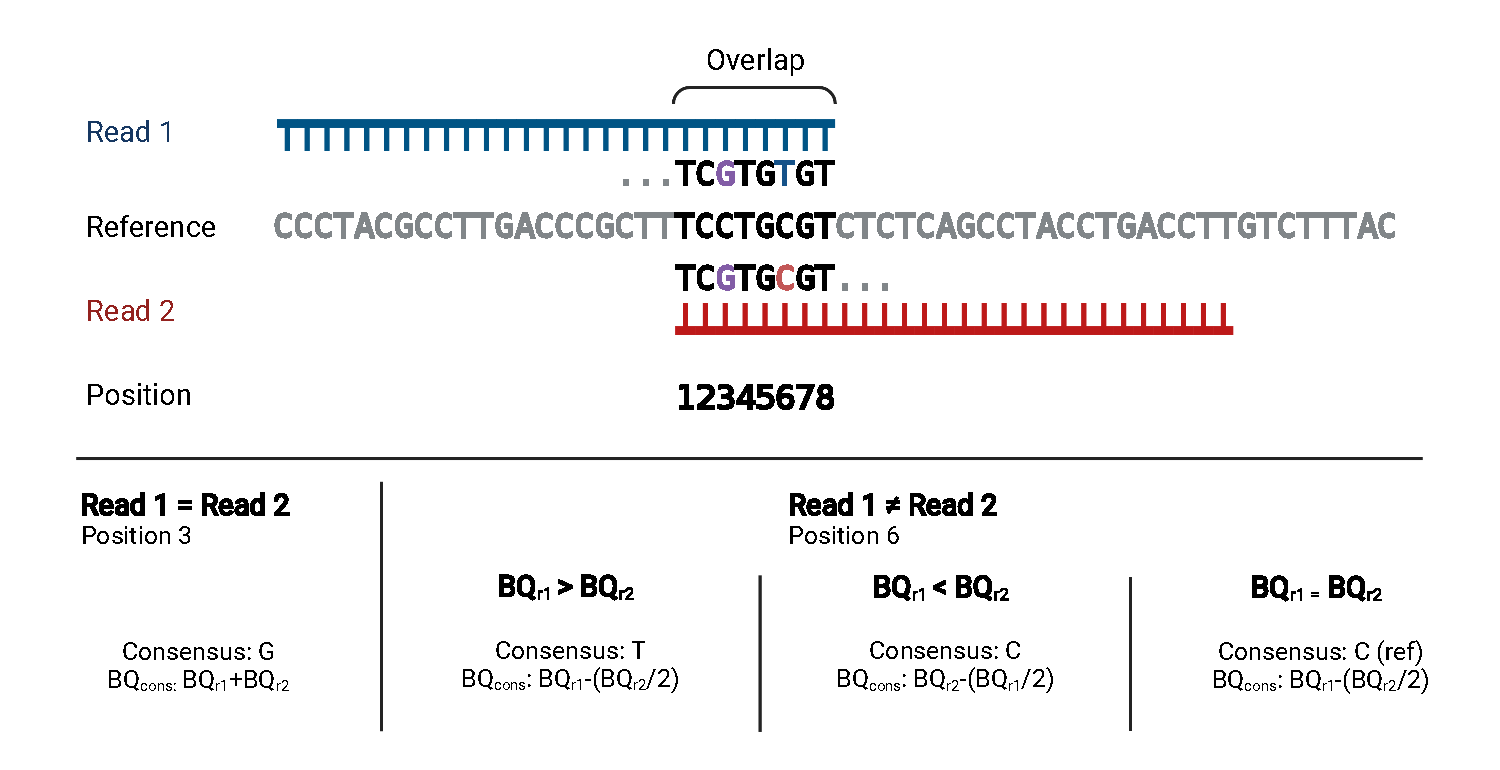
\includegraphics[width=.99\linewidth]{Figures/ConsensusMethodMisMatchFinder.pdf}
\caption[Schematic of consensus computation method for overlapping reads]{Schematic of consensus computation method for overlapping reads in MisMatchFinder; Read 1 and Read 2 depict two overlapping paired end reads aligned to the reference sequence; Positions in the overlap are numbered for later referral; Read positions agreeing with the reference are coloured black, positions differing from the reference but agreeing in both reads are coloured purple (position 3) and differences between reads are coloured in the respective read colours (blue and red, position 6); Calculation for the resulting base quality (BQ$_{cons}$ for each possibility is shown as formulas)}\label{fig:mmf-consensus}
\end{figure}

This method however also reduces the available data by restricting the analysis to areas where reads are overlapping. Due to the fragment size distribution of ctDNA a paired end sequencing with 100bp  read length will in most cases lead to an overlap of at least 45 nucleotides (\autoref{intro-sec:ctDNA}) and with 150bp most ctDNA fragments will be almost entirely covered by both reads in theory. However due to soft-clipping and incomplete alignment, this number will be lower in reality.
In our tests, the restriction leads to on average 18 nucleotides (min:~14bp max:~25bp std.dev.:~1.45) being retained in the analysis from a read on average for a 100bp read in real world data. This however means that with a read depth of 8-10x $\approx$80\% of the genome will be covered by the overlap of at least one read pair.



\subsection[Germline filtering]{Germline filtering - exclusion of normal variation}
\label{mmf-sec:germline}

To further enable the \autoref{mmf-sec:concept} claim that the germline is a very small constant, we need to remove as many mismatches as possible, which stem from germline variants. For this purpose, I built a zarr \cite{Miles2021} based storage system from the gnomAD database (v.3.1) \cite{Karczewski2020} using scikit-alel \cite{Miles2021a}.
A in-depth explanation of the generation as well as a script for for an end user can be found in \autoref{ch-mmfAppendix:germlineFilter}.

This then allows very precise filtering of known germline variants sites from the analysis. The method allows the specification of an allele frequency to consider a variant to be filtered, however as baseline, it will filter all sites, which were detected in any sample in gnomAD. This even includes sites with low quality variants, as these are signs for sequencing or mapping complications, which will most likely interfere with our method as well.


\subsection[Count normalisation]{Count normalisation - not everyone has the same chances}
\label{mmf-sec:countNorm}
Finally when having filtered all ``noise`` mismatches from the dataset, we can aggregate all mismatches to oligo-nucleotide counts. With this step also comes the classification of 
directly neighbouring mismatches as DBS, which are counted as separate entities. SBS and DBS both can be used to identify underlying biological mutational processes, but they have very different signatures associated with them \cite{Alexandrov2020}. The counts formed this way are influenced by the background frequency of their reference oligo-nucleotides in the analysed genomic region. As the frequencies of di- and tri-nucleotides are not uniform in the genome, the chance for a mismatch found in an ``AAA`` reference contex is almost seven times higher than a mismatch in ``CGC`` (\autoref{A:mmf:tab:tricounts}, \autoref{A:mmf:tab:dicounts}). To reduce this bias towards high frequency oligo-nucleotides, I implemented a count normalisation step.

First the di- and tri-nucleotides in the analysed regions are counted using the supplied reference without any black-listed and/or only in white-listed regions. These counts are then either used to directly weight the observed mismatch counts, which leads to a more uniform distribution of mismatches, or by building a fraction of observed oligo-nucleotides and the total counts in the genome (\autoref{A:mmf:tab:tricounts}, \autoref{A:mmf:tab:dicounts}), the weighting achieves an approximation of how the counts would be distributed over the whole genome. These two options are available with \lq\emph{--normaliseCounts}\rq~ for the approximation to full genome. By also adding \lq\emph{--flatNormalisation}\rq~ only the observed counts are used for normalisation.

\subsection[Signature deconvolution]{Signature deconvolution - find the original signal}
\label{mmf-sec:sigDeconv}
The deconvolution of the involved signatures from known set of signatures is equivalent to finding the minimal distance between $m$ as the observed number of mismatches in each oligo-nucleotide context (a vector of length 96) and $\textbf{S}w$, where $\textbf{S}$ is the matrix of oligo-nucleotide defined contributions for each signature, resulting in a matrix of $96 \times k$ with $k$ being the number of known signatures. Lastly, $w$ is the vector of weights of each signature, which we want to estimate. 

\begin{align}
 \text{minimise:} & \quad (m - \textbf{S}w)^T(m - \textbf{S}w)
 = m^Tm - w^T\textbf{S}^Tm - m^T\textbf{S}w + w^T\textbf{S}^T\textbf{S}w \label{mmf-eq:optim1}\\
 \text{with:} & \quad \sum_j w_j = 1 \quad \text{and} \quad \boldsymbol{\forall} j ~ w_j \geq 0 \label{mmf-eq:requirements}
\end{align}
\myequation[\ref{mmf-eq:optim1}]{MisMatchFinder: optimisation for signature weights}
\myequation[\ref{mmf-eq:requirements}]{MisMatchFinder: optimisation function restrictions}

\autoref{mmf-eq:optim1} can then be written as 

\begin{equation}
\text{minimise:} \quad - m^T\textbf{S}w + \frac{1}{2}w^T\textbf{S}^T\textbf{S}w
\label{mmf-eq:optim2}
\end{equation}
\myequation[\ref{mmf-eq:optim2}]{MisMatchFinder: quadratic programming formula}

With the same restrictions as shown in \autoref{mmf-eq:requirements}. These equations and the idea to solve it with quadratic programming (QP) have been taken from \textcite{Lynch2016}, the iterative linear models (ILM) solving approach was adapted from deconstructSigs \cite{Rosenthal2016}. Both methods are reimplemented in python in MisMatchFinder, using the quadprog package \cite{McGibbon2021} for QP and a translation of the R code of deconstructSigs for ILM.

MisMatchFinder allows the use of either QP or ILM, as they in many cases produce very similar results \cite{Lynch2016}. The default method is QP however, even though ILM is the more interpretable method and is the more parsimonious method, because with the increased number of signatures, in the latest work by \textcite{Alexandrov2020}, ILM does not lead to the right signatures if the signal is not strong enough but QP seems to be more stable (\autoref{fig:mmf-ILMerror}).

\begin{figure}[!ht]
\centering
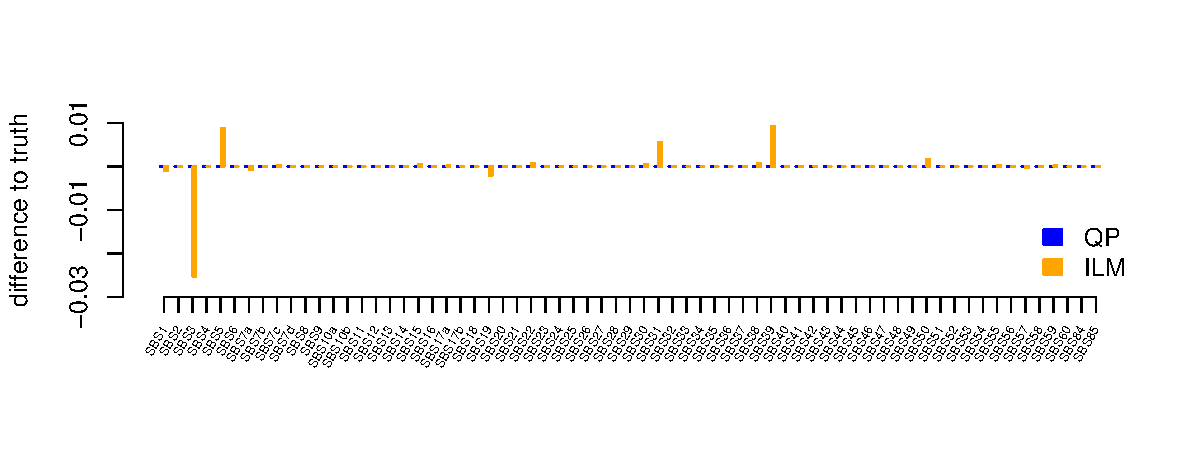
\includegraphics[width=.99\linewidth]{Figures/lowInputSignalDeconv.pdf}
\caption[Distance of deconvolution methods from truth]{Distances of the estimated weights generated with ILM and QP from the true weight used as input; Truth is a synthetic count sample with (SBS1: 0.25; SBS3: 0.05; SBS5: 0.46; SBS7a: 0.1; SBS19: 0.03; SBS21: 0.01; SBS31: 0.08; SBS57: 0.02;)}\label{fig:mmf-ILMerror}
\end{figure}
 
The combinatorial problem in ILM, already shown by \textcite{Lynch2016}, seems to be especially strong with ``wide`` signatures like SBS3 (\autoref{fig:sig7a}) and low signature contribution. That makes it less useful for our approach, as we expect low tumour purity and therefore low somatic signature signals in cfDNA, but even with ILM as deconvolution method impacts the detection of SBS7a less than the detection of SBS3. especially for SBS3 the weight for ILM will only be assigned with sufficient signal (15 and 20 mutations per megabase respectivly for for SBS7a and SBS3) where QP allows a more linear increase in signal, even at lower levels. In contrast ILM will assign more weight overall than QP once the signal reaches a certain threshold (\autoref{fig:mmf-methodDifferences}). This means, that ILM will be better for high powered signal, but less effective for the more subtle differences we expect from ctDNA.

The deconvolution method might be a spot for further optimisation by creating a custom deconvolution system adjusted for ctDNA detection.

For the rest of this chapter, unless specified differently, the results shown will use the QP deconstruction method.

\todo[color=green,inline]{maybe move the simulation description here}


\subsection{Signature detection}
\label{mmf-sec:sigdetection}
Signature deconvolution with QP will lead to non negative signature weights for almost all of the signatures when using MisMatchFinder derived counts, however a positive signature does not necessarily signal the activity of this process in a tumour capacity due to the normal somatic mutation background and germline residual signal (\autoref{mmf-sec:germlineArtifacts}). To enable calling of significantly active signatures in samples, we developed a z-score based system, which uses the distribution of each signature weight in the healthy population as a background.

The z-score of each patient samples ($p$) signature weight $w$ was calculated per signature $s$, using the mean $\overline{w}_h(s)$ and standard deviation $\sigma_h(s)$ of the weight $w$ of all healthy samples for the respective signature $s$ (\autoref{eq:sigZScore}).

\begin{equation}
\forall s \in Signatures,\ \forall p \in Patients:\ \text{z-score}(s,p) := \frac{w_s(p) - \overline{w}_h(s)}{\sigma_h(s)}
\label{eq:sigZScore}
\end{equation}
\myequation[\ref{eq:sigZScore}]{MisMatchFinder: z-score calculation per signature and patient}

This allowed the prioritization of significantly changed signatures in the tumour samples with regards to our healthy background depending on the desired application. A higher z-score cut off will increase specificity at the cost of sensitivity. For any of our results we considered a z-score $\geq 4$ as a cut off. This very conservative measure accounts for the possibility of a non-representative sampling process in the healthy sample set, as well as reduces false positive calls, which are highly problematic in the cancer context.

